% Author: Izaak Neutelings (March 2020)
\documentclass[border=3pt,tikz]{standalone}
\usepackage{amsmath} % for \dfrac
\usepackage{bm} % \bm
\usepackage{physics}
\usepackage{tikz,pgfplots}
\usepackage[outline]{contour} % glow around text
\usetikzlibrary{angles,quotes} % for pic (angle labels)
\usetikzlibrary{calc}
\usetikzlibrary{decorations.markings}
\usetikzlibrary{patterns,snakes}
\tikzset{>=latex} % for LaTeX arrow head
\contourlength{1.6pt}
\usepackage{xcolor}
\colorlet{Bcol}{violet!90}
\colorlet{BFcol}{red!60!black}
\colorlet{Scol}{green!60!black}
\colorlet{veccol}{green!45!black}
\colorlet{Icol}{blue!70!black}
\colorlet{mucol}{red!90!black}
\tikzstyle{BField}=[->,thick,Bcol]
\tikzstyle{current}=[->,Icol] %thick,
\tikzstyle{force}=[->,thick,BFcol]
\tikzstyle{vector}=[->,thick,veccol]
\tikzstyle{mu vector}=[->,thick,mucol]
\tikzstyle{spin}=[->,very thick,Scol]
\tikzstyle{velocity}=[->,very thick,vcol]
\tikzstyle{charge+}=[very thin,draw=black,top color=red!50,bottom color=red!90!black,shading angle=20,circle,inner sep=0.5]
\tikzstyle{charge-}=[very thin,draw=black,top color=blue!50,bottom color=blue!80,shading angle=20,circle,inner sep=0.5]


\begin{document}


% MAGNETIC MOMENT ELECTRON + SPIN
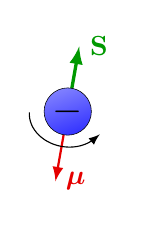
\begin{tikzpicture}
  \def\re{0.3}
  \def\ang{80}
  %\draw[dashed] (\ang-180:2.5*\re) -- (\ang:3.5*\re);
  \draw[mu vector] (0,0) -- (\ang+180:3*\re) node[right] {$\vb*{\mu}$}; %_\mathrm{e}
  \draw[spin] (0,0) -- (\ang:2.8*\re) node[right] {$\vb{S}$};
  \draw[charge-]
    (0,0) circle (\re) node[scale=1.4] {$-$};
    %node[right=10] {$\mathrm{e}^-$};
  \draw[->,rotate=\ang-90]
    (0,-0.2*\re)++(-175:{1.6*\re} and {1.3*\re}) arc (-175:-35:{1.6*\re} and {1.3*\re})
    --++ (50:0.3*\re);
\end{tikzpicture}


% MAGNETIC MOMENT POSITRON + SPIN
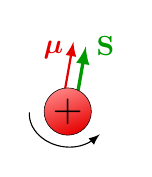
\begin{tikzpicture}
  \def\re{0.3}
  \def\ang{80}
  %\draw[dashed] (\ang-180:2.5*\re) -- (\ang:3.5*\re);
  \draw[mu vector] (-0.28*\re,0) --++ (\ang:3*\re) node[below=3,left=0] {$\vb*{\mu}$}; %_\mathrm{e}
  \draw[spin] (0.28*\re,0) --++ (\ang:2.8*\re) node[right] {$\vb{S}$};
  \draw[charge+]
    (0,0) circle (\re) node[scale=1.4] {$+$};
    %node[right=10] {$\mathrm{e}^+$};
  \draw[->,rotate=\ang-90]
    (0,-0.2*\re)++(-175:{1.6*\re} and {1.3*\re}) arc (-175:-35:{1.6*\re} and {1.3*\re})
    --++ (50:0.3*\re);
\end{tikzpicture}



\end{document}